\documentclass[10pt,twocolumn,letterpaper]{article}
%\usepackage[review]{cvpr}
%\usepackage[final]{cvpr}
\usepackage[pagenumbers]{cvpr} % To force page numbers, e.g. for an arXiv version


\usepackage[utf8]{inputenc} % allow utf-8 input
\usepackage{url}            % simple URL typesetting
\usepackage{amsfonts}       % blackboard math symbols
\usepackage{nicefrac}       % compact symbols for 1/2, etc.
\usepackage{graphicx}
\usepackage{wrapfig}

% Include other packages here, before hyperref.
\usepackage{graphicx}
\usepackage{amsmath}
\usepackage{amssymb}
\usepackage{booktabs}
\usepackage{placeins}
\usepackage{tabularx}
\usepackage{multirow}


%
% --- inline annotations
%
\usepackage[dvipsnames]{xcolor}
\newcommand{\red}[1]{{\color{red}#1}}
\newcommand{\todo}[1]{{\color{red}#1}}
\newcommand{\TODO}[1]{\textbf{\color{red}[TODO: #1]}}
% --- disable by uncommenting  
% \renewcommand{\TODO}[1]{}
% \renewcommand{\todo}[1]{#1}

% It is strongly recommended to use hyperref, especially for the review version.
% hyperref with option pagebackref eases the reviewers' job.
% Please disable hyperref *only* if you encounter grave issues, e.g. with the
% file validation for the camera-ready version.
%
% If you comment hyperref and then uncomment it, you should delete
% ReviewTempalte.aux before re-running LaTeX.
% (Or just hit 'q' on the first LaTeX run, let it finish, and you
%  should be clear).
\definecolor{cvprblue}{rgb}{0.21,0.49,0.74}
\usepackage[pagebackref,breaklinks,colorlinks,citecolor=cvprblue]{hyperref}

\def\confName{ar$\xi$iv}
\def\confYear{2023}

%%% Add PDF metadata to help others organize their library
%%% Once the PDF is generated, you can check the metadata with
%%% $ pdfinfo template.pdf
\hypersetup{
	pdftitle={Beyond the Final Linear Layer},
	pdfauthor={Michael Majurski, David Chapman},
	pdfkeywords={AI,Semi-Supervised,Classification,FixMatch},
}



\begin{document}
	
	% \title{GmmMatch: Enhancing Semi-Supervised Learning with a Generative Gaussian Mixture Model Final Layer}
	% \title{The Use of a Generative Gaussian Mixture Model Final Layer For Enhancing Deep Semi-Supervised Learning}
	% \title{Enhancing Deep Semi-Supervised Learning via a Generative Gaussian Mixture Model Final Layer}
	% TODO fix the wording to harp on the Generative vs Discrimitative nature.
	\title{Enhancing Semi-Supervised Learning with a Generative Gaussian Mixture Model Final Layer}
	
	%\title{Training a final activation layer with the method of moments, and its application to semi-supervised learning.}
	
	\author{Michael Majurski\\
		Information Technology Lab, NIST\\
		University of Maryland, Baltimore County\\
		%	100 Bureau Dr. Gaithersburg MD, 20899\\
		{\tt\small michael.majurski@nist.gov}
		% For a paper whose authors are all at the same institution,
		% omit the following lines up until the closing ``}''.
	% Additional authors and addresses can be added with ``\and'',
	% just like the second author.
	% To save space, use either the email address or home page, not both
	\and
	Sumeet Menon\\
	University of Maryland, Baltimore County\\
	{\tt\small sumeet1@umbc.edu}
	\and
	Parniyan Farvardin\\
	University of Miami\\
	{\tt\small pxf291@miami.edu}
	\and
	David Chapman\\
	University of Miami\\
	{\tt\small dchapman@cs.miami.edu}
}

\maketitle




% SCOPE paper review notes that I need to make sure i also address
% 1- The novelty of the proposed method is very limited. Many previous works have explored pseudo-labeling approaches based on local neighborhood density such as TSSDL [3], LPD [4], DASO [5].
%2- The paper is not well-written, the method sections lacks clarity, the experiments section is badly organized and lacks important details.
%3- The experimental evaluation is not convincing due to:
%3.1- Lack of comparison with important baselines such as: Smooth Neighbors on Teacher Graphs [1], Interpolation Consistency Training [2], FlexMatch [7], TSSDL [3], LPD [4], DASO [5], Dash[6].
%3.2- The performance gains obtained with 250 labels and 4000 labels on cifar10 are not significant. A similar case of very limited performance gains on CIFAR100 with 2500 and 4000 labels.
%3.3- The ablation study findings show that dropping the Gaussian filter or KNN filter do not cause a drop in performance of the proposed method.
%This raises the issue of the need for using both filters as the performance of SCOPE does not degrade when either component/filter is dropped.
%
%[1] Smooth neighbors on teacher graphs for semi-supervised learning, CVPR 2018.
%[2] Interpolation consistency training for semi-supervised learning, Neural Networks 2022.
%[3] Transductive semi-supervised deep learning using min-max features, ECCV 2018.
%[4] Label propagation for deep semi-supervised learning, CVPR 2019.
%[5] Distribution- aware semantics-oriented pseudo-label for imbalanced semi-supervised learning, CVPR 2022.
%[6] Dash: Semi-supervised learning with dynamic thresholding, ICML 2021.
%[7] Boosting semi-supervised learning with curriculum pseudo labeling, NeurIPS 2021.

%1. The results are reported only on Cifar-10 and Cifar-100 datasets. Considering that the initial training only is performed for 1024 epochs, is it scalable for larger datasets?
%2. The paper seems to have been rushed and has several writing issues:
%* The beginning of the related work section is repetitive with the introduction. Where as experts in this area probably know what they refer to, non-experts are left to wonder.
%* The variables X and Y in Section 1.1 are not defined
%* "After the model is m_1 and m_2" is grammatically incorrect... I think it is meant to say "After the models m_1 and m_2..."
%* X_L, Y_L in equation 1 are not defined. Are they supposed to be X_S and Y_S
%* In Section 4.1, it states "One must further assume that sample independence". This assumption is not justified and I might think likely wrong (despite the authors claiming its is "common".)
%
%Please compare with more recent approaches in this area. For example:
%[1] FlexMatch: Boosting Semi-supervised Learning with Curriculum Pseudo Labeling, NeurIPS 2021
%[2] FreeMatch: Self-adaptive Thresholding for Semi-supervised Learning, ICLR 2023


\begin{abstract}
	Semi-Supervised Learning (SSL) leverages an abundance of unlabeled data to improve deep learning based model performance under limited training data regimes.
	This paper presents a novel extension to any image classification architecture which improves accuracy in low-label regimes by enhancing class inlier determination. 
	We demonstrate our method by extending the FixMatch \cite{sohn2020fixmatch} training scheme with our novel final layers. 
	We present two semi-parametric final layers of differing complexity (a) the Axis Aligned GMM (AAGMM) layer, and (b) an equal variance version we call KMeans. % of AAGMM we call KMeans.
	Both layers are integrated into the network architecture as regular fully differentiable modules which are trained via backprop (not Expectation Maximization).
	Importantly, these novel layers exhibit both discriminative and generative properties, enhancing their capability to characterize inlier data; improving pseudo-labeling performance. 
	We also introduce and evaluate a series of class-wise embedding constraints based on the Method of Moments (MoM) \cite{pearson1936method} in order to fit the parameters of our semi-parametric latent prior.  
	These methods match published SOTA 250 label CIFAR-10 \cite{cifar10} accuracy and come close to matching the recently improved SOTA in the 40 label regime without the significant increase in model complexity of other modern SOTA methods \cite{zheng2023simmatchv2}.
	%Our method achieves 94.8\% and 94.2\% accuracy with 250 and 40 CIFAR-10 labels respectively.
	%Our code is available at: \url{https://github.com/*} % \url{https://github.com/mmajurski/ssl-gmm}
\end{abstract}


\section{Introduction}

\TODO {(majurski) purge bibliography of arxiv pre-prints where possible, replacing with their peer reviewed equivalents}

%\begin{figure}[ht]
%	\centering
%	\includegraphics[width=0.9\linewidth]{example-image-a}
%	\caption{High level overview of our method. \TODO {(majurski) Create this figure.}}
%	\label{fig:schema}
%\end{figure}

\begin{figure}[ht]
	\centering
	\subfloat{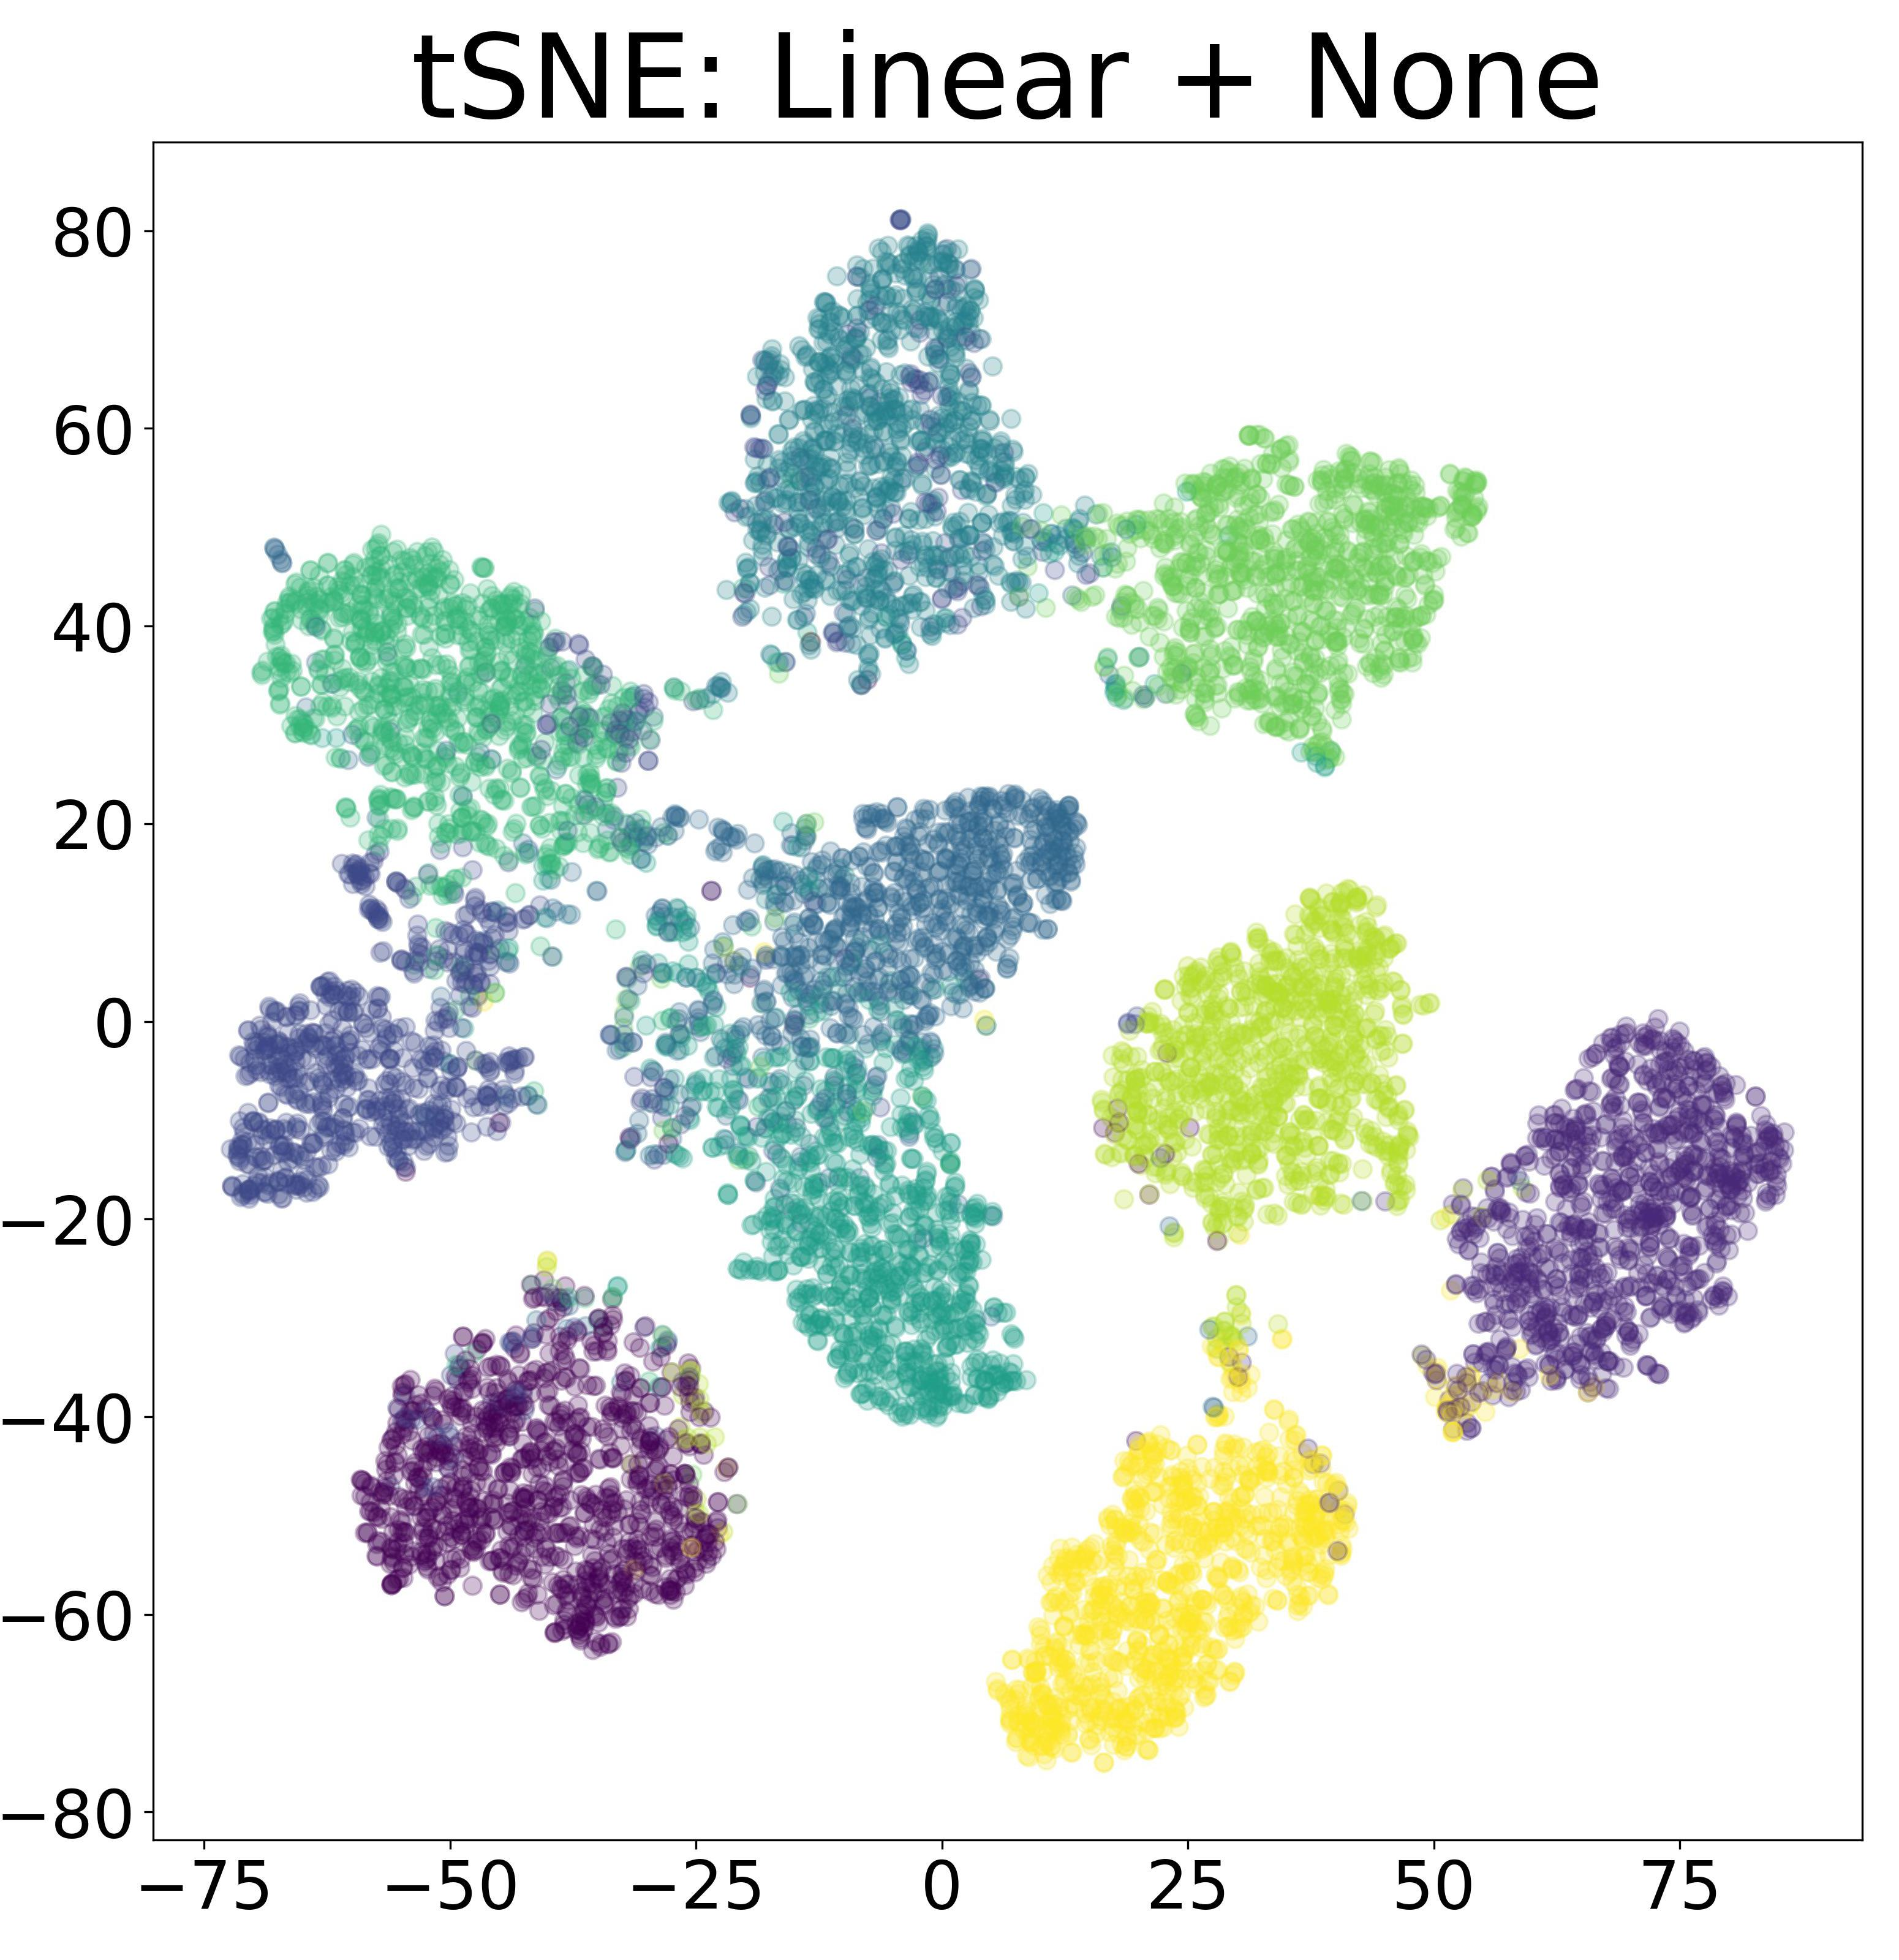
\includegraphics[width=.5\columnwidth]{figures/id-00000001-tsne.jpg}}
	\subfloat{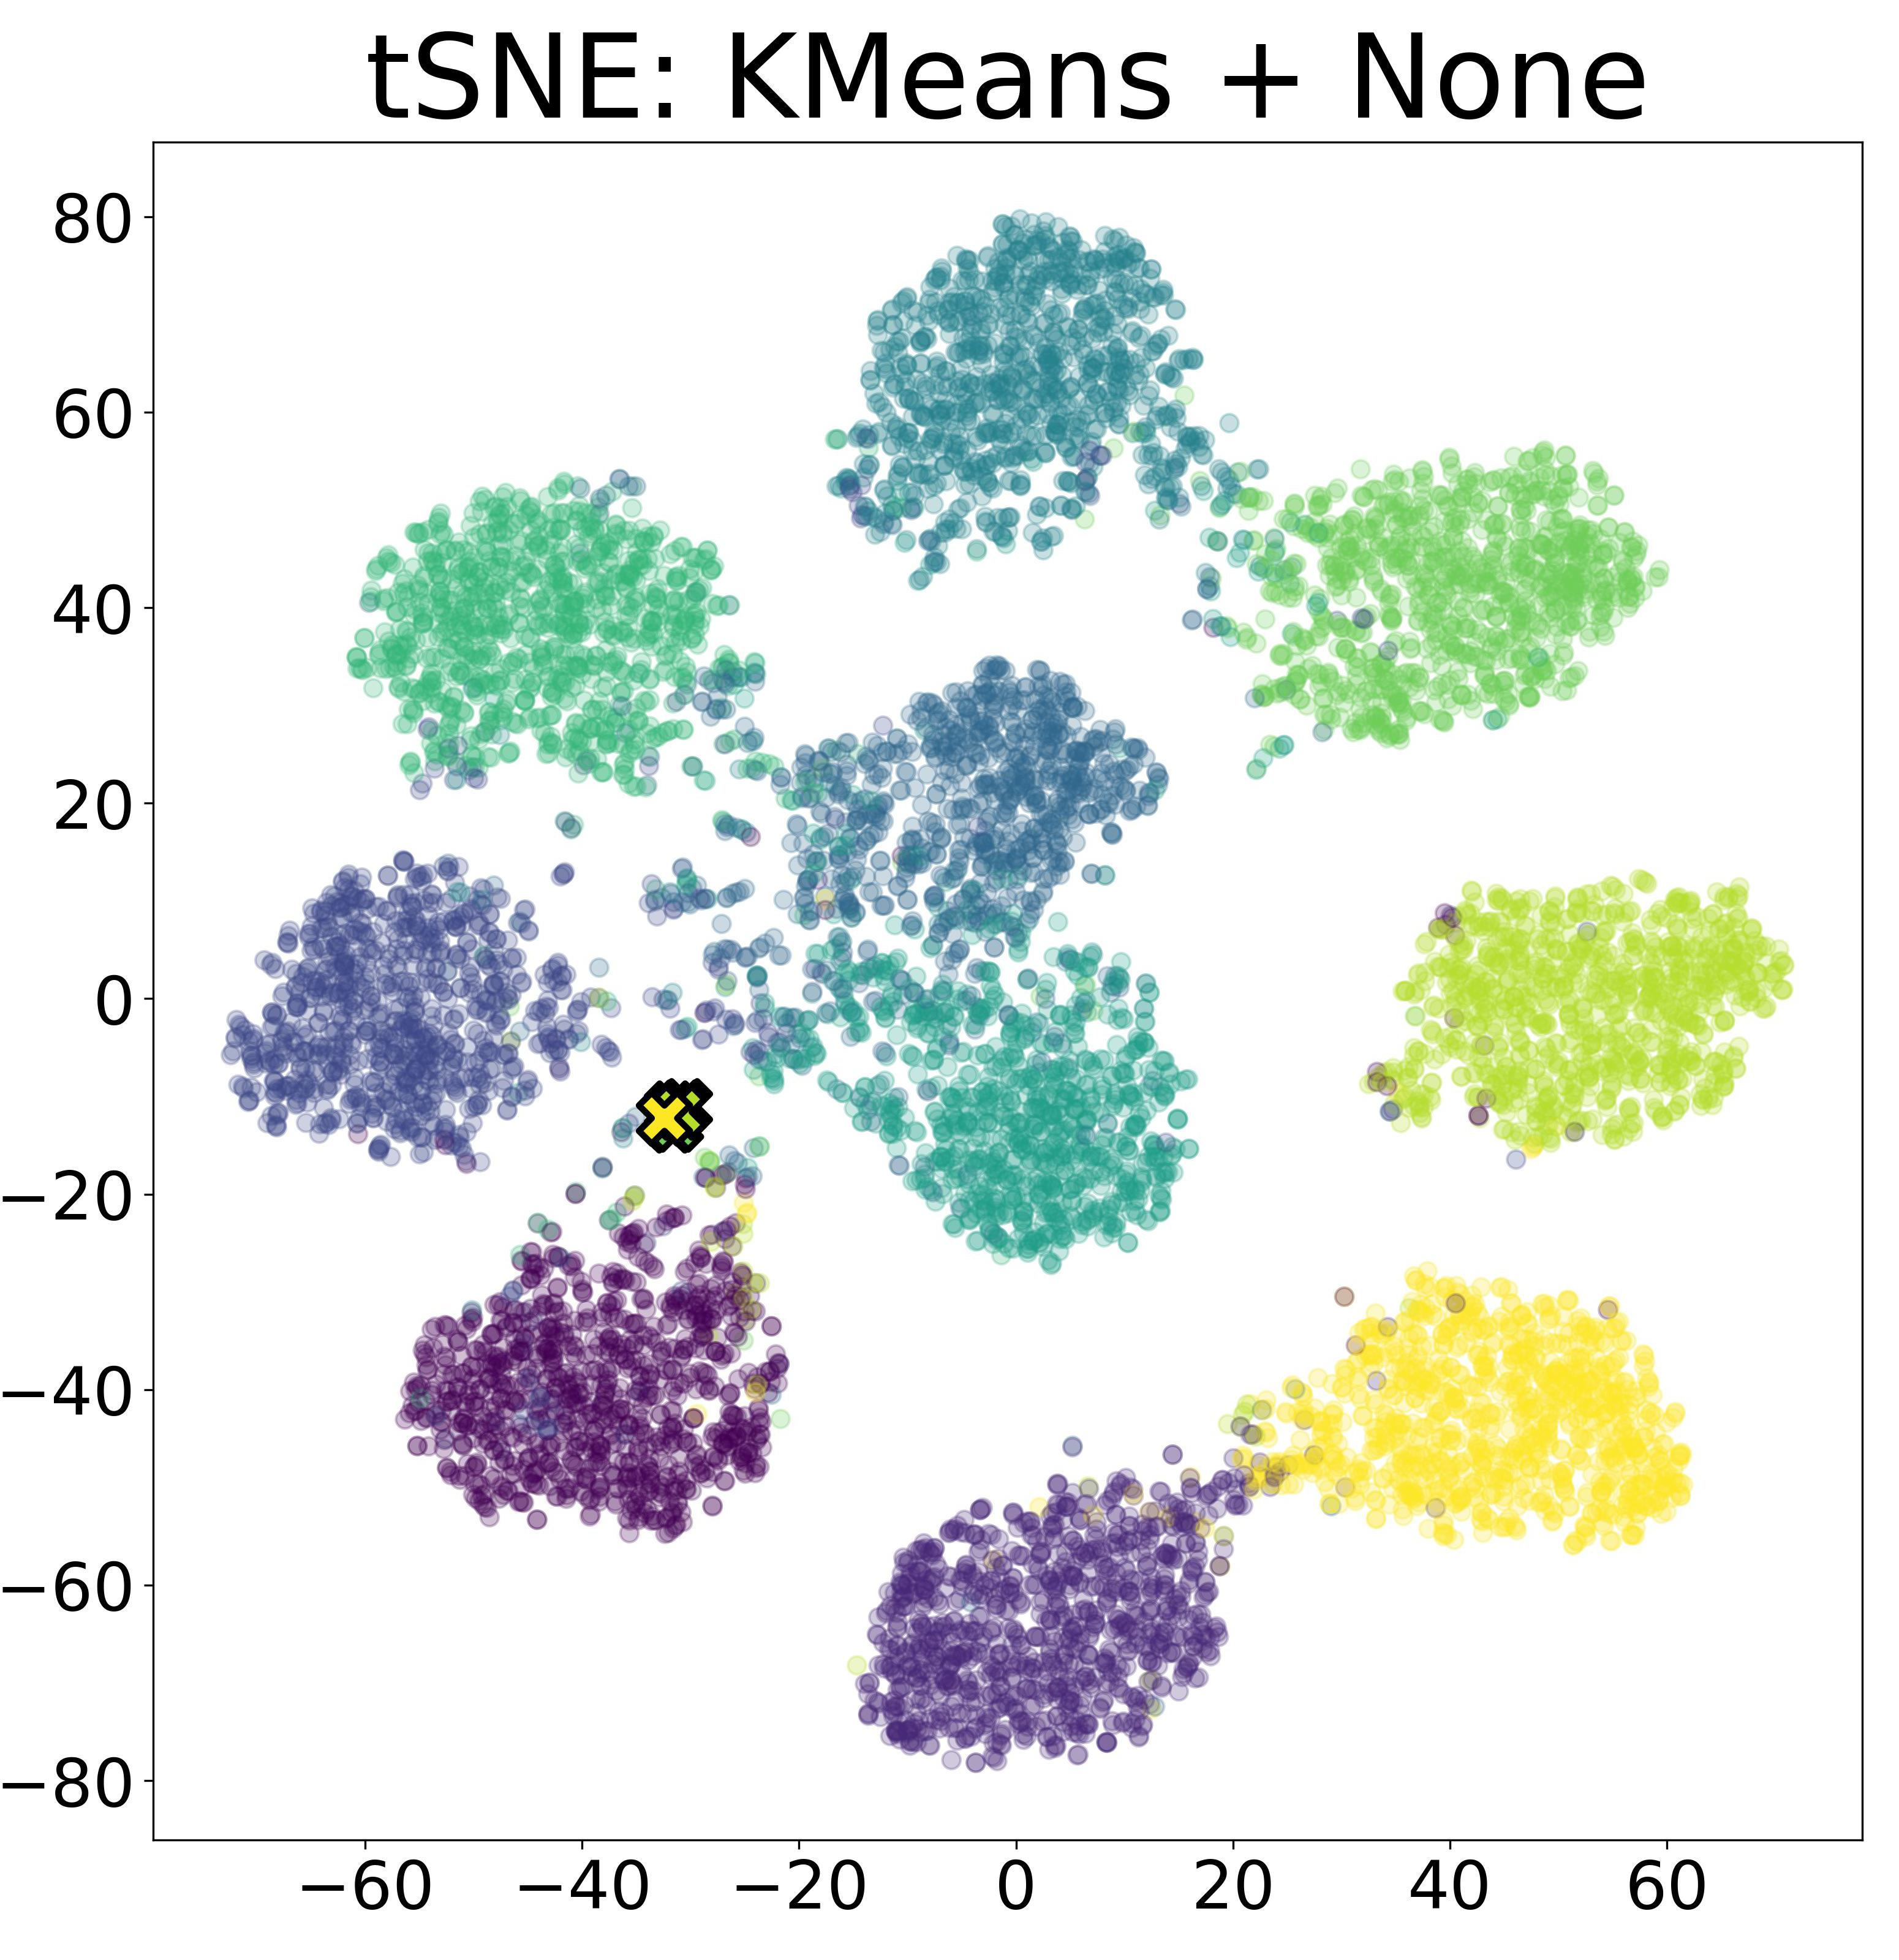
\includegraphics[width=.5\columnwidth]{figures/id-00000013-tsne.jpg}}
	\\
	\subfloat{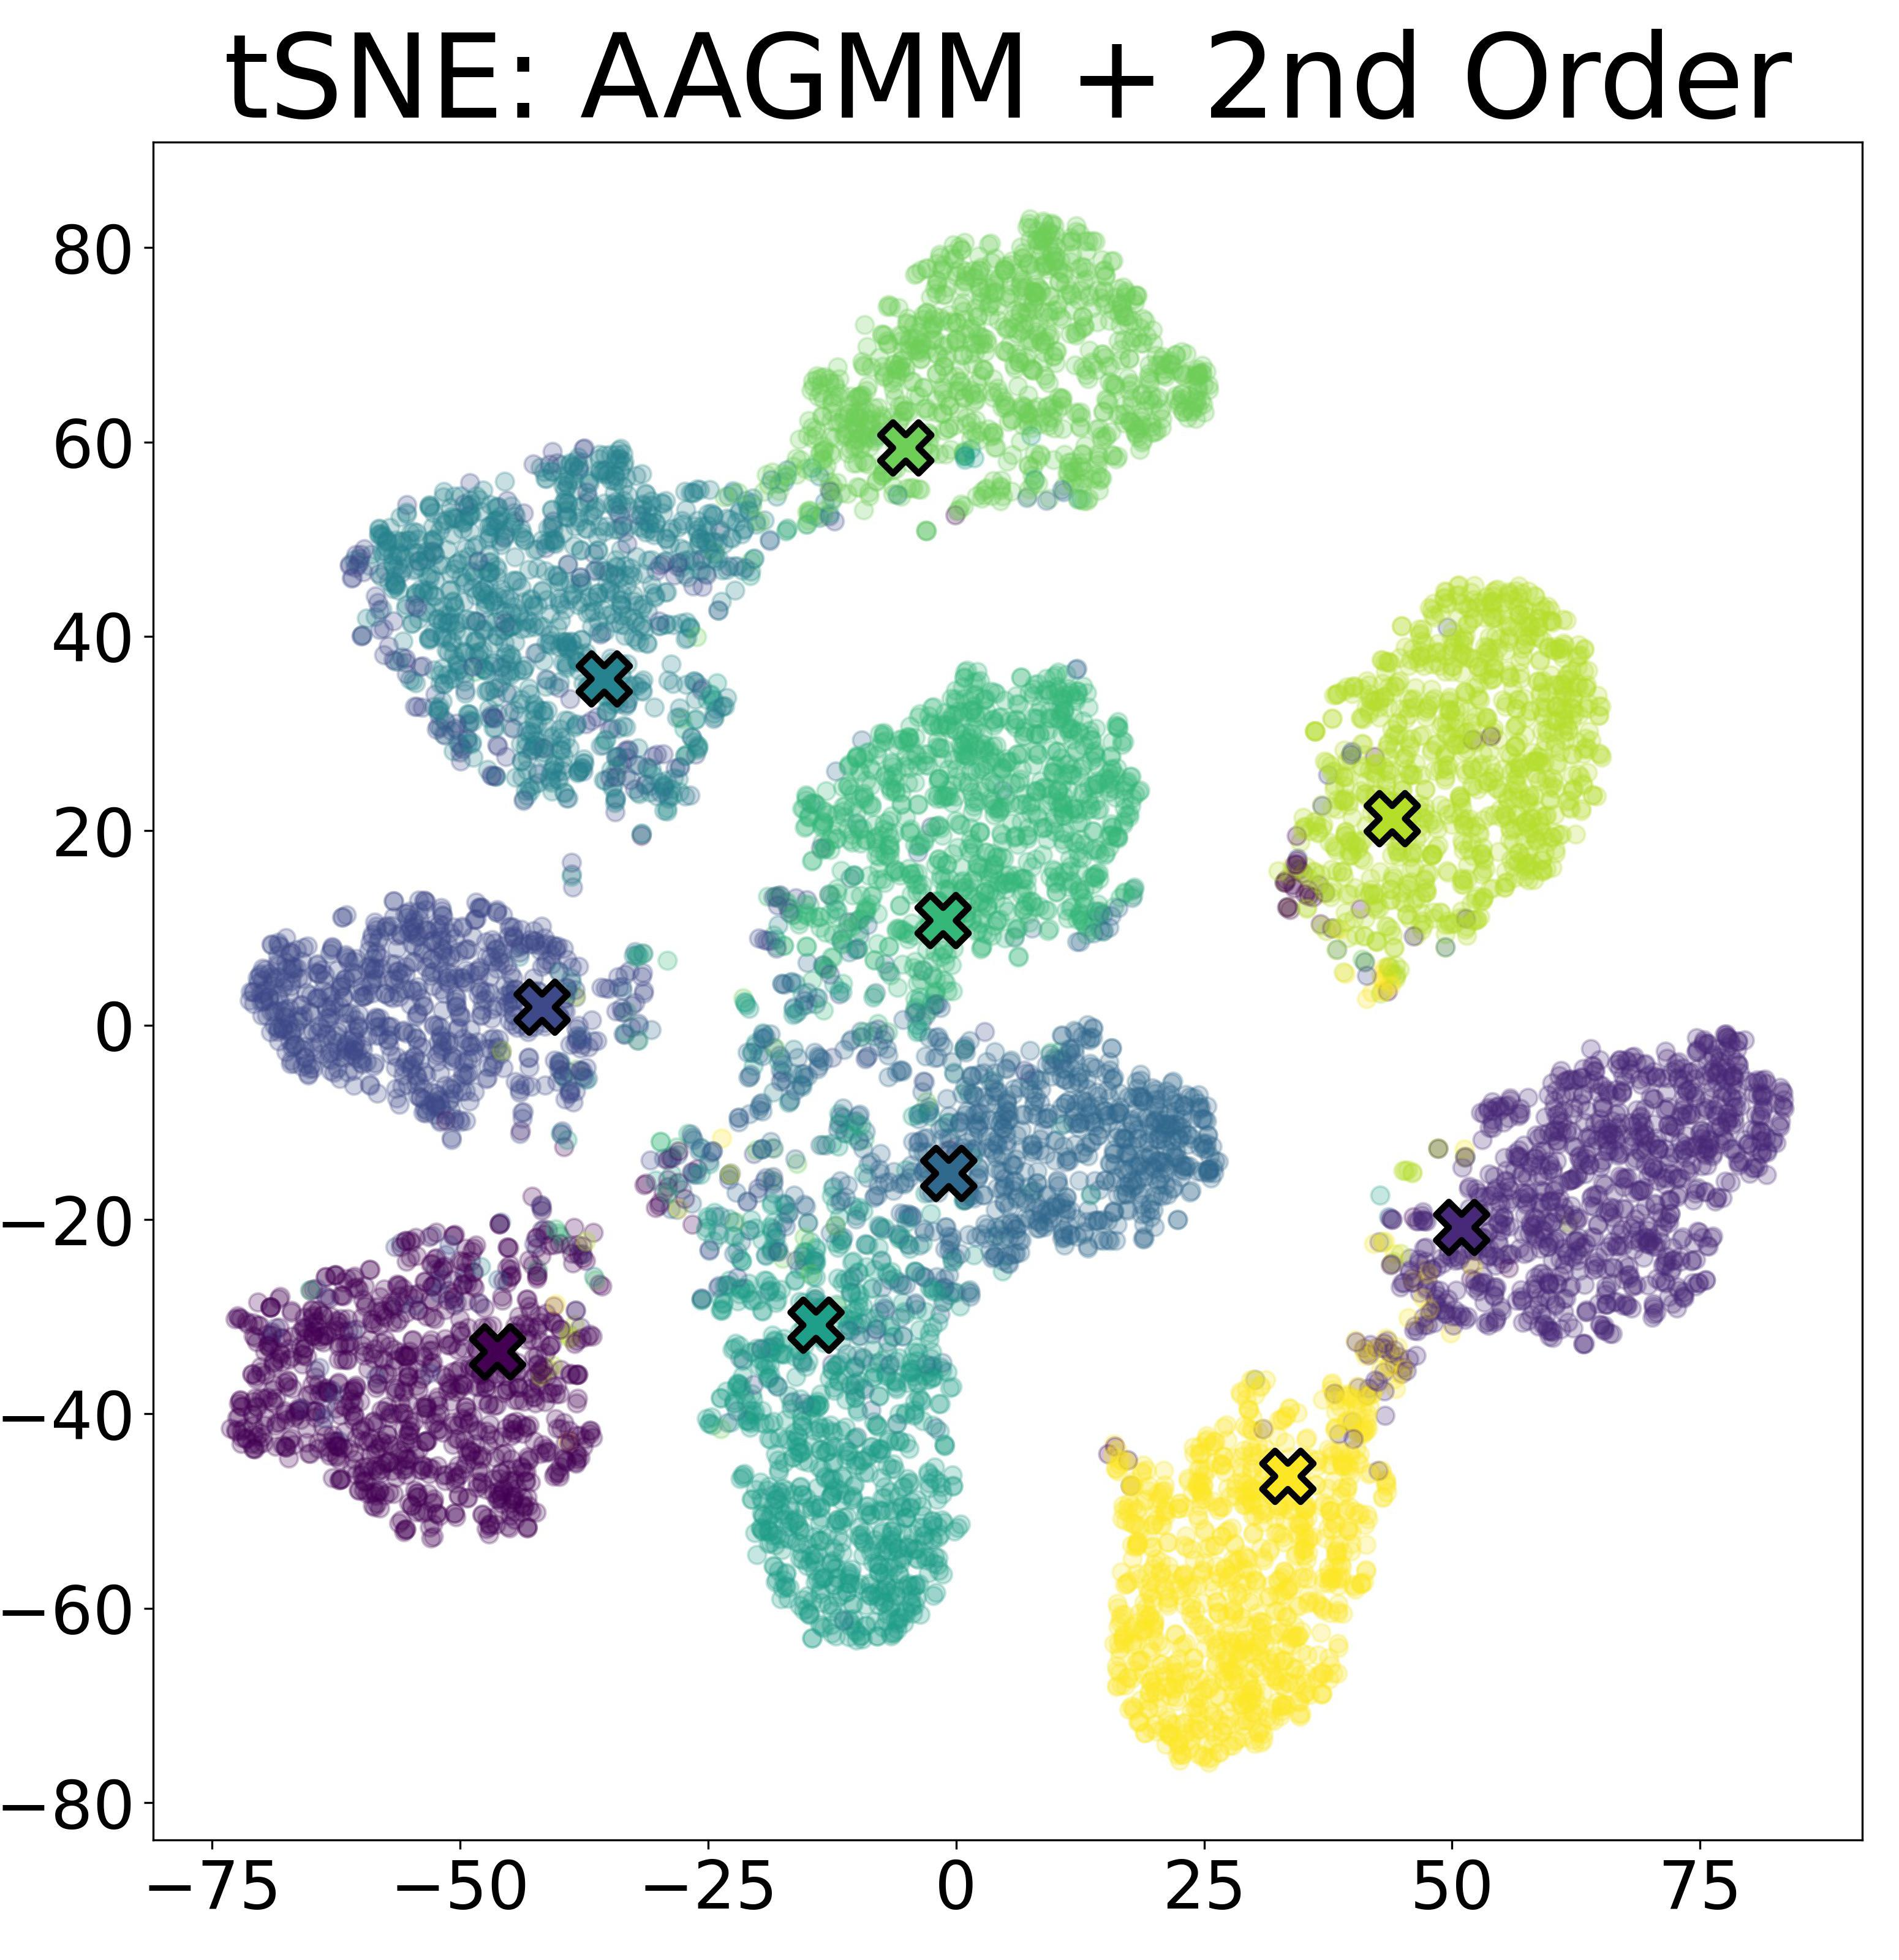
\includegraphics[width=.5\columnwidth]{figures/id-00000054-tsne.jpg}}
	\subfloat{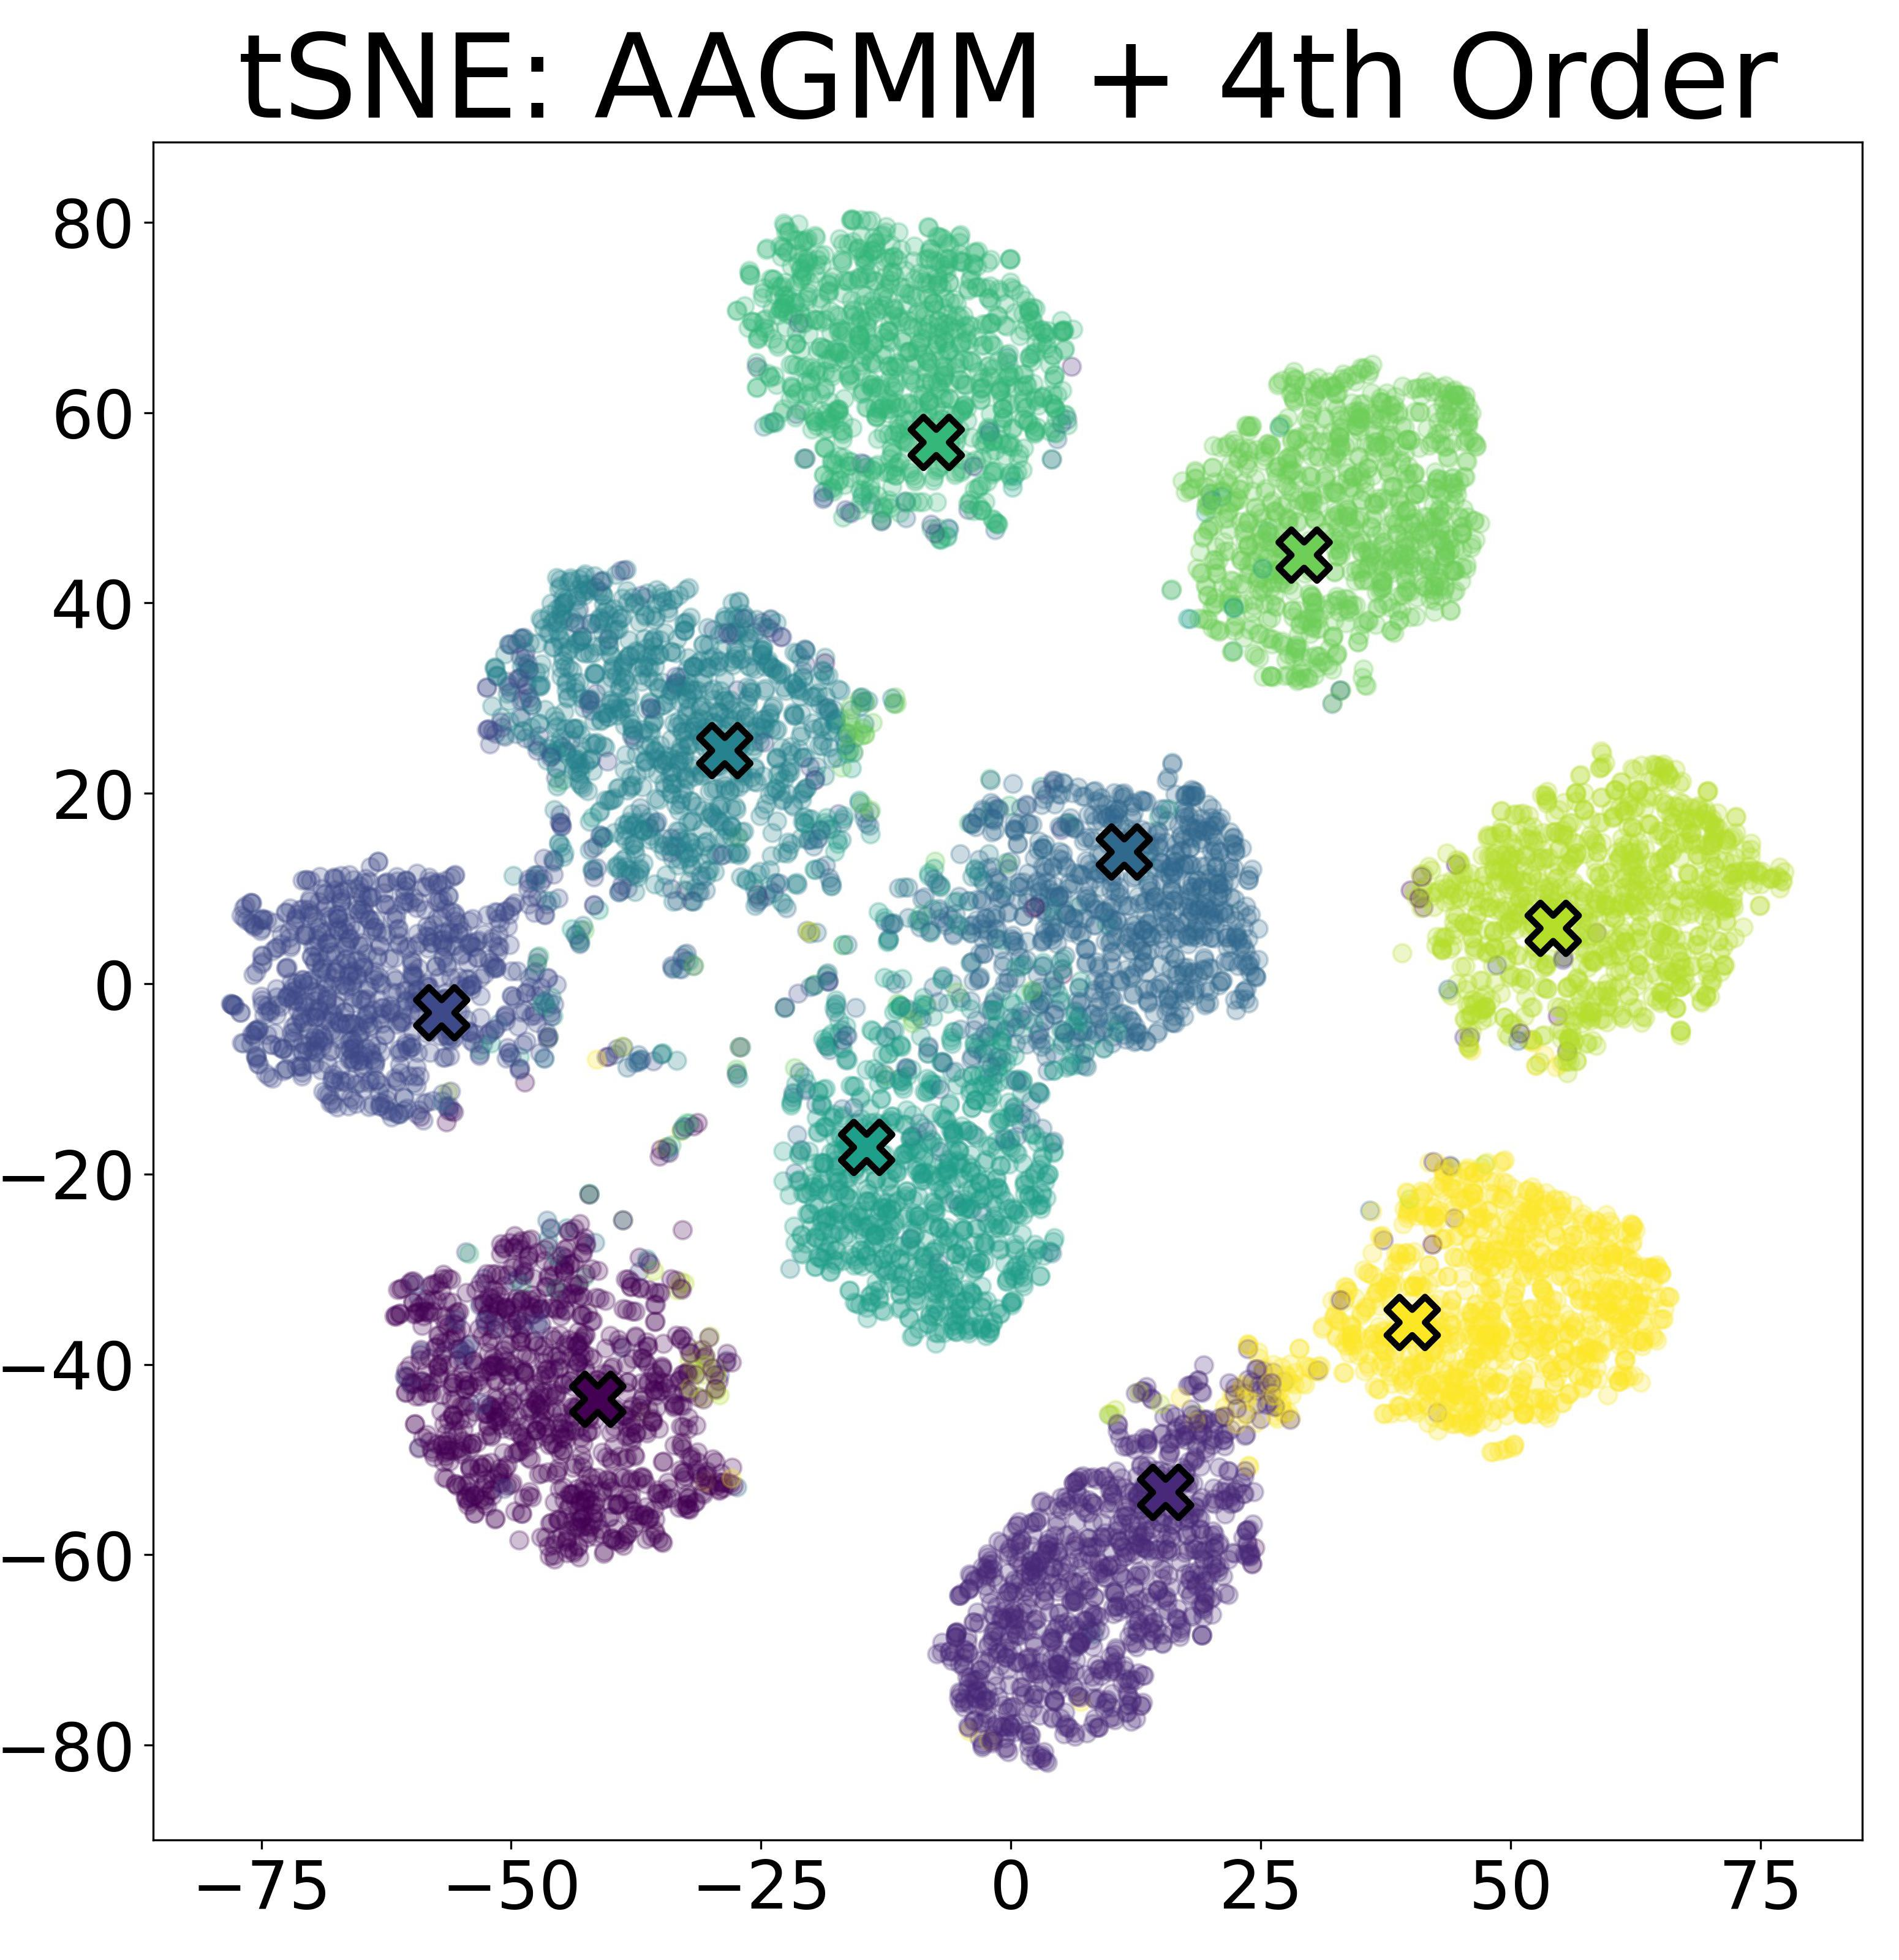
\includegraphics[width=.5\columnwidth]{figures/id-00000021-tsne.jpg}}
	
	%	\includegraphics[width=0.9\linewidth]{example-image-a}
	\caption{t-SNE plot of the latent embedding space for various final network layers with different Method of Moments embedding constraints.} 
	\label{fig:schema}
\end{figure}

SSL leverages an abundance of unlabeled data to improve deep learning based model performance under limited training data regimes \cite{zhu2022introduction,li2019safe,hady2013semi}.
Image classification has become a playground for exploring novel SSL ideas.
The early successes of deep learning based methods relied on large annotated datasets to enable models to learn the relevant features to perform the task, i.e. image classification build on top of ImageNet \cite{deng2009imagenet}.
With data annotation becoming a significant bottleneck, especially in application domains outside of the standard benchmarks, another learning paradigm was needed.

There are several flavors of SSL.
Contrastive learning methods leverage the intuition that similar instances should be close in the representation space, while different instances are farther apart \cite{yang2022class,li2021comatch}.
Consistency regularization borrows the intuition that modified views of the same instance should have similar representations and predictions \cite{sohn2020fixmatch,lee2022contrastive,zhang2021flexmatch,kim2022conmatch}.
Pseudo-labeling methods like FixMatch \cite{sohn2020fixmatch} fall within the consistency regularization domain.

This work argues that pseudo-labeling methods can be improved with better calibration of the network logits used to filter the pseudo-labels into reliable and unreliable. 
This is equivalent to improving the accuracy of class inlier determination.
Neural networks are known to be overconfident in their predictions \cite{wei2022mitigating}, and this affects the pseudo-labeling process. 
Potentially allowing for the inclusion of more incorrect pseudo-labels any specific logit threshold would otherwise have.
This work demonstrates the better calibrated replacements for a models final linear layer can improve the final accuracy of pseudo-labeling based SSL algorithms in very label scarce regimes. 
This work proposes:

% TODO write up what the motivation for our method was, why do the things we do...? (not because they are easy, but because they are hard...) Most papers have an inciting incident in the intro which outlines the hypothesis that X is a problem, and we addressed that via Y to improve the results by Z.
\begin{enumerate}
	\item Replacing the final linear (fully connected) layer of the neural network with either an axis-aligned differentiable Gaussian Mixture Model (AAGMM) or an equal variance version named KMeans trained via back prop, both of which have explicit modeling of class cluster centroids. 
	\item We explore various constraints on how the embedding space should be structured by adding penalties if the per-class clustering does not conform to between 0 and 4 of the first gaussian moments being identity/zero \cite{pearson1936method}.
	\item We demonstrate that increasing the specificity of how the embedding space should be structured negatively impacts model performance. 
\end{enumerate}

This paper explores the impacts of replacing the final linear layer of a network with a generative model and embedding space constraints.
This combination demonstrates improvements in final model accuracy when using pseudo-labeling methods where very few annotations are available.
We demonstrate this methodology using the standard CIFAR-10 benchmark dataset with 40 and 250 labels\cite{cifar10}. %) and CIFAR-100 (400 and 2500 label) benchmarks \cite{cifar10}. 
Additionally, we explore and demonstrate that high level prescriptive constraints on the embedding space produce significantly worse outcomes than allowing the embedding space to take on whatever emergent structure the training process produces. 
Finally, because the embedding constraint penalties are applied to all unlabeled data and not just the valid pseudo-labels, our method extracts training signal from every unlabeled data point, unlike FixMatch \cite{sohn2020fixmatch} and other methods which only learn from the valid pseudo-labels.


% TODO CE masked where any truely low logit values are kept, but those midling are left alone.? I.e keep CE <0.1 but ignore those 0.1 < x < 0.95. cite chen2023boosting and rizve2021defense and kim2019nlnl for the idea. I.e. keep the strong negative PL in the CE term. chen2023boosting uses topk, instead of thresholds. 

% TODO perform study with best mothod (i.e. aa_gmm_d1 or kmeans with l2) and show impact of PL threshold and the model impurity rate compared to baseline fixmatch (fc). Gerenate plot of impurity for FM vs gmm over the first 100-200 epochs?]


\section{Related Work}

% TODO cite and compare against xu2021dash and zhang2021flexmatch and wang2022freematch for curiculum pseudo-labeling and how that can orthogonally improve SSL

% TODO compare our method to lee2022contrastive which uses explicit cluster centers, and draws both the valid and non valid PL to the cluster center, just like we do, we just don't have a contrastive element like they do

Semi-Supervised learning has shown great progress in learning high quality models, in some cases matching fully supervised performance for a number of benchmarks \cite{zhang2021flexmatch}.
The goal of SSL is to produce a trained model of equivalent accuracy to fully supervised training, with vastly reduced data annotation requirements.

\subsection{Pseudo-Labeling}
Self-supervised learning was among the initial approaches employed in the context of semi-supervised learning to annotate unlabeled images. 
This technique involves the initial training of a classifier with a limited set of labeled samples and incorporates pseudo-labels into the gradient descent process, exceeding a predefined threshold \cite{yarowsky1995unsupervised, mcclosky2006reranking, olivier2006semi,zhai2019s4l,livieris2019predicting,rosenberg2005semi,menon2020deep}. 
A closely related method to self-training is co-training, where a given dataset is represented as two distinct feature sets \cite{blum1998combining}. 
These independent sample sets are subsequently trained separately using two distinct models, and the sample predictions surpassing predetermined thresholds are utilized in the final model training process \cite{blum1998combining,prakash2014survey}.
A notably advanced approach to pseudo-labeling is the Mean Teacher algorithm \cite{tarvainen2017mean}, which leverages exponential moving averages of model parameters to acquire a notably more stable target prediction. 
This refinement has a substantial impact on enhancing the convergence of the algorithm.

% TODO update related works with some of the ideas from the FREEMATCH papers related works on enhancing the single tau threshold


\subsection{Consistency Regularization}

Consistency regularization operates on the premise that when augmenting an unlabeled sample, its label should remain consistent. 
This approach implicitly enforces a smoothness assumption, promoting coherence between unlabeled samples and their basic augmentations \cite{xie2020unsupervised}. 
In other words, the model should be able to predict the unlabeled sample $x$ exactly the same way it predicts the class for $Augmented(x)$ \cite{berthelot2019mixmatch,sohn2020fixmatch,berthelot2019remixmatch,mustafa2020transformation}. 
In addition to evaluating image-wise augmentations, recent research has demonstrated that incorporating class-wise and instance-based consistencies yields superior performance outcomes \cite{zheng2022simmatch,li2021comatch}. 
Similarly, using consistencies between augmentations, of the predictions and low-dimensional embeddings of the strong and weak augmentations of the unlabeled images in a graph based setup has shown improvement over class-wise and instance-based consistencies \cite{zheng2023simmatchv2}.
Finally, pseudo-labeling filtering based on consistence between strongly augmented views, gaussian filtering and embedding based nearest neighbor filtering shows convergence improvement \cite{kim2022conmatch,menon2022semisupervised}.

\subsection{Embedding Clustering/Constraints}

% TODO talk about the paper which find linear layers end up being nearest neighbor assignment (with cone away from origin structure) in the embedding space (Majurski cannot find the citation, so anyone who remembers what this paper was titled please leave a comment here.

Several papers have attempted to enhance the quality of pseudo-labels to either improve the final model accuracy, improve the rate of convergence, or avoid confirmation bias \cite{arazo2020pseudo}.
Rizve et al. \cite{rizve2021defense} explores how uncertainty aware pseudo-label selection/filtering can be used to reduce the label noise.
Incorrect pseudo-labels can be viewed as a network calibration issue \cite{rizve2021defense} where better network logit calibration might improve results \cite{Xing2020DistanceBased}.
Other work has attempted to improve the pseudo-labeling process by imposing curriculum \cite{zhang2021flexmatch} or by including a class-aware contrastive term \cite{yang2022class}.
Previous work has leveraged the concept of explicit class cluster centers for conditioning semantic similarity \cite{zheng2022simmatch}.
Recent work has extended purely clustering based methods like DINO \cite{caron2021emerging} into semi-supervised methods \cite{fini2023semi}.

% TODO {(chapman) find and include citations you were reading about embedding constraints. You mentioned this in the meeting on the 17th.}

% TODO talk about SimMatch embedding constraint via semantic seimilarity?

\TODO {(majurski) compute the delta in PL accuracy for two runs with same seed. Base Fixmatch, and our best.}

\section{Methodology}

In this section, we explore our proposed replacement final layers and our embedding space constraints.
FixMatch \cite{sohn2020fixmatch} is a simple, well performing, SSL algorithm.
As such, it serves as a good comparison point for exploring the effect of our contributions.
Our methodology is based upon the published FixMatch \cite{sohn2020fixmatch} algorithm, with identical hyper-parameters unless otherwise stated.
We extend FixMatch with an early-stopping condition when the model has not improved for 40 epochs (where epoch size is defined as 1024 batches), and with 2 learning rate reductions by a factor of $0.2$ instead of configuring a fixed number of training epochs with a cosine learning rate decay.
Additionally, we employ a cyclic learning rate scheduler to vary the learning rate by a factor of $\pm2.0$ within each epoch to make training less dependent upon exact learning rate value.

Both the linear layer replacements and the embedding constraints explored herein represent increasing levels of prescription about how the final embedding space should be arranged compared to a traditional linear layer.
The idea of leveraging clusters in embedding space is not new \cite{caron2018deep,caron2020unsupervised,enguehard2019semi}, but we extend the core idea with a novel differentiable model with learned cluster centroids and GMMs.

\subsection{Alternate Final Layers}

A limitation of traditional final activation layers such as linear+softmax is that they are fully discriminative; i.e. they estimate the posterior $p(Y|X)$, but do not attempt to model the sample distribution $p(X)$ or the joint probabilities $p(Y,X)$. 
To overcome this limitation, we present two semi-parametric final activation layers (a) the Axis Aligned GMM (AAGMM) layer, and (b) an equal variance version of AAGMM that we henceforth call the KMeans activation layer due to the similarity of the objective function with a gradient based KMeans.

These activation layers are fully differentiable and integrated into the neural network architecture as a module in the same way as a traditional final linear layer. 
As such, they do not require or depend on external training and do not use expectation maximization.
They are drop in replacements for the final linear layer.

Importantly, these activation layers exhibit both discriminative and generative properties. 
The neural network model $F(X;\theta_F)$ transforms the data $X$ into a latent space $Z = F(X;\theta_F)$, and the final activation layer estimates the probability densities $p(X)$, $p(Y;X)$ and $p(Y|X)$ by fitting a parametric model to the latent representation $Z$.

\subsubsection{Axis Aligned Gaussian Mixture Model Layer}

The AAGMM layer defines a set of $K$ trainable clusters, one cluster per label category. 
Each cluster $k=1 \dots K$ has a cluster center $\mu_k$ and cluster covariance $\Sigma_k$. 
The prior probability of any given sample $X_i$ is defined by the mixture of cluster probability densities over the latent representation $Z_i$ as follows,

\begin{equation}
	\begin{aligned}
		\label{eq_px}
		&p(X_i) = \sum_{k=1}^K \mathcal{N} (Z_i, \mu_{k}, \Sigma_k)
		\\[10pt]
		&\textit{where} \quad Z_i = F(X_i, \theta_F)
	\end{aligned}
\end{equation}

Where $\mathcal{N}(Z_i, \mu_k, \Sigma_k)$ represents the multivariate gaussian pdf with centroid $\mu_k$ and covariance $\Sigma_k$. 
AAGMM is axis aligned because $\Sigma_k$ is a diagonal matrix, as such the axis-aligned multivariate normal pdf simplifies to the marginal product of Gaussians along each of the $D$ axes as follows,

\begin{equation}
	\begin{aligned}
		\mathcal{N} (X_i, \mu_{k}, \Sigma_k) &=  \prod_{d=1}^D \frac{1}{\sigma_{k,d}\sqrt{2 \pi}} exp \Big( \frac{Z_{i,d} - \mu_{k,d}} {\sigma_{k,d}} \Big)^2 \\[10pt]
		&\textit{where} \quad \sigma^2_{k,d} = \Sigma_{k,d,d}
	\end{aligned}
\end{equation}

As there is one cluster per label category, the joint probability for sample $i$ with label assignment $k$, $p(Y_{i,k},X_i)$ is the given by the normal pdf of the $k^{th}$ cluster,

\begin{equation}
	\label{eq_pyx}
	p(Y_{i,k},X_i) = \mathcal{N} (Z_i, \mu_{k}, \Sigma_k) \end{equation}

By simple Bayesian identity, the posterior probability $\hat{Y}_k=p(Y_{k}|X_i)$ can therefore be inferred from eq \ref{eq_px} and \ref{eq_pyx} as follows,

\begin{equation}
	\hat{Y}_{i,k} = p(Y_{i,k}|X_i) = \frac{p(Y_{i,k}, X_i)}{p(X_i)}
\end{equation}

%The $\mu_k$ and $\Sigma_k$ are trainable parameters and are trained as part of the gradient descent procedure.  The posterior probabilities $\hat{Y}_{i,c} = p(Y_i=c|X_i)$ are calculated by making use of a Bayesian identity $p(b|a) = p(b,a)/p(a)$, along with mutual exclusion of the label categories as follows,
%
%\begin{equation}
%p(Y_i=c|X_i) = \frac{p(Y_i=c,X_i)}{\sum_{j=1}^C}
%\end{equation}

%as follows,
%
%\begin{equation}
%\begin{aligned}
%\mathcal{N} (X_i, \mu_{k}, \Sigma_d) = \\
%(d \pi)^{- \frac{d}{2}}det(\Sigma_k)^{- \frac{1}{2}} \\
%exp\Big(-\frac{1}{2}(X_i-\mu_k)^t \Sigma^{-1} (X_i-\mu_k)\Big)
%\end{aligned}
%\end{equation}

The AAGMM layer is implemented as a normal PyTorch \cite{pytorch} module.
It has two parameters updated by backprop.
(1) the explicit cluster centers, a $num\_classes \times embedding\_dim$ matrix randomly initialized, and
(2) the diagonal elements of the $Sigma$ matrix, randomly initialized in the range $[0.9, 1.1]$, which contains the diagonal elements of the GMM Sigma matrix for each cluster.

\subsubsection{KMeans Layer}

We also implement a KMeans final layer which is a more restrictive form of the AAGMM layer, in the sense that we impose an additional constraint that the gaussian covariance matrix $\Sigma_k$ for each cluster center $k$ is the $[D \times D]$ identity matrix. 
This constraint yields spherical cluster centers similar to how the traditional KMeans algorithm also assumes spherical clusters.
%It is notable, that in both cases, the AAGMM layer and the KMeans layer are not trained using the KMeans algorithm, or with any form of expectation maximization.  Rather, they are trained by gradient descent as a fully integrated module within the network architecture.  

%The KMeans activation layer defines a set of C trainable cluster centers, one cluster center per label category.  This layer is called a KMeans layer because, like KMeans, it makes use of equal-variance gaussians to define the prior $p(X)$.  However, it is not trained using the KMeans algorithm, but instead by making use of cross entropy loss as part of the neural network model.  We define $K$ $D$-dimensional cluster centers $\mu_1 \ldots \mu_K$, one center per label category.  This constitutes a generative model, where the prior probability of any given sample $X_i$ is defined in terms of the cluster centers as follows

The KMeans layer is also implemented as a normal PyTorch \cite{pytorch} module.
It has just one learnable parameter updated by backprop: the explicit cluster centers, a $num\_classes \times embedding\_dim$ matrix randomly initialized.

See the published codebase for implementation details about AAGMM and KMeans.




\subsection{Method of Moments Embedding Constraints}

We also introduce and evaluate a series of embedding constraints based on the Method of Moments (MoM) \cite{pearson1936method} in order to fit the parameters of our semi-parametric latent prior.  
As such, we calculate the latent prior $p(X_i)$ as in equation \ref{eq_px}, which is then used to infer the posterior $p(Y_{i,k}|X_i)$.  As usual, the posterior is trained using cross entropy loss.  
But, if one were to omit embedding constraints, then it is possible that the model could learn a good decision boundary for the posterior but without actually modeling the latent prior.
%The MoM solve this issue by constraining the prior to fit the latent distribution.

Our model is semi-parametric, because the prior is a parametric model of the latent distribution $Z$ which is the result of a neural network feature extraction $F(X;\theta)$. 
As such, attempting to fit the GMM directly to $Z$ using Maximum Likelihood (ML) or simple Expectation Maximization (EM), is not appropriate, because doing so would fail to learn an appropriate feature space for discrimination.
MoM solves these problems and is an appropriate strategy for semi-parametric models including ours.

%MoM constraints typically use the L2 norm to constrain the.  % TODO clarification for this sentence?
The MoM relies on the use of \textit{consistent estimators}, as these asymptotically share sample and population statistics.
Assume that $z$ is a finite sample of $n$ elements drawn from infinite population $Z$, then a series of $P$ well-behaved sample statistics $g_p$ should very closely approximate their $k$ population statistic as follows,

\begin{equation}
	\forall p=1 \dots P \quad
	\frac{1}{n} \sum_{i=1}^n g_p(z_i) \approx E(g_p(Z))
\end{equation}

We can therefore constrain the latent representation of our model to approximate an independent joint Gaussian distribution. 
In the univariate gaussian case, the $p^{th}$ order centralized moment constraint is the following.

\begin{equation}
	E\left[ (Z-\mu)^p \right] = 
	\begin{cases} 
		0 &  \text{if} \; p \; \text{is odd} \\
		\sigma^p(p - 1)!! & \text{if} \; p \; \text{is even}
	\end{cases}
\end{equation}

By this formula, the univariate unit gaussian has mean $0$, standard deviation $1$, skew $0$, and kurtosis 3.

In the joint multivariate case, each dimension is independent by definition.  As such, if we redefine $Z$, $\mu$, and $p$ to be all $D$ dimensional, then the centralized joint gaussian moment can be defined as follows,

\begin{equation}
	E\left[g_p(Z - \mu)\right] = E\left[ \prod_{d=1}^D (Z_d - \mu_d)^p_d \right]
\end{equation}

Due to independence of the axes, this moment can be represented as a product of univariate moments of the individual gaussians as follows,

\begin{equation}
	E\left[ \prod_{d=1}^D (Z_d - \mu_d)^p_d \right] = \prod_{d=1}^D E\left[ (Z_d - \mu_d)^p_d \right]
\end{equation}

The error (loss) term associated with the embedding constraint for any moment $p$ is equal to the L2 difference between the sample and population statistics as follows,

\begin{equation}
	\varepsilon_p = \left( \frac{1}{n} \sum_{i=1}^n g_p(z_i) - E(g_p(Z)) \right)^2
\end{equation}

Some moments are more important than others, and must be weighted more heavily.  
For example, first order moments are simply the sample mean, and should be given the greatest weight as an embedding constraint.  
The second order moments form a sample covariance matrix, which ideally should be equal to the identity matrix, but the diagonal terms should be given greater weight than the off-diagonal terms.  
This is because, in a $D \times D$ covariance matrix, there are $D(D-1)$ off diagonal terms, but only $D$, diagonal terms.  
The $p^{th}$ order sample moments form a $p-1$ dimensional hyper-covariance matrix, with terms residing on the intersection of anywhere between $0$ and $p-1$ hyper-diagonals.  
In order to prevent over-representation of off-diagonal terms, and encourage representation of on-diagonal terms, the loss function for any given moment term is inversely proportional to the number moment terms that share the same number of hyper-diagonals.  
This heuristic weighting scheme ensures that the overall contribution of each moment order is not overly influenced by the off-diagonal terms, and that the error weighting is therefore diagonally dominant.

%Define $Z^k$, $X^k$, $Y^k$, and $\hat{Y}^k$, as the latents, samples, labels, and posteriors for the elements that are predicted to reside with label $Y^k$ as follows,
%
%\begin{equation}
%(Z^k, X^k, Y^k, \hat{Y}^k) = \{(Z_i, X_i, Y_i, \hat{Y}_i) \; \; | \; \;  \underset{\rm j}{\rm argmax} \; \hat{Y}_{i,j}=k \}
%\end{equation}

%\subsubsection{Moment1}
%
%This constraint encourages the learned cluster means to have zero distance to the ovserved centroids. 
%Define $pred_k$ as the set of indices $i=1 \dots K$ such that are predicted to be of category $k$ as follows,
%
%\begin{equation}
%	pred_k = \{i \;\; | \;\; \underset{j}{argmax} \; \hat{Y}_{i,j} \; \text{is equal to} \; k\}
%\end{equation}
%
%This embedding constraint ensures that cluster centers $\mu_k$ approximate the sample distribution of latent points that are part of cluster $k$, $E(Z_i|\hat{Y}_{i,k}=1)$. 
%The $L2$ norm is used as a loss function to constrain cluster centers as follows,
%
%\begin{equation}
%	\begin{aligned}
	%		\mathcal{L}_{L2} = \sum_{k=1}^K \Bigm\lvert\Bigm\lvert \mu_k - \bar{Z} \Bigm\lvert\Bigm\lvert_2 \\[5pt]
	%		\textit{where} \quad \bar{Z} = E_{i \in pred_k}Z_i
	%	\end{aligned}
%\end{equation}
%
%\subsubsection{Moment2}
%
%Additionally, the L2 norm was also used to constraint the cluster covariance terms to the identity matrix.
%Although the AAGMM assumes a diagonal covariance matrix $\Sigma_k$, the mini-batch sample estimate of the covariance may exhibit off-diagonal terms, which represent
%
%\subsubsection{Moments 3 and 4}
%
%Moment3 encourages clusters to have zero skew. 
%% TODO {fill in with math if required? Or just remove the subsubsections and talk about all the moments in a few paragraphs}
%
%Moment4 encourages cluster kurtosis to be the identity matrix. 
%% TODO {fill in with math if required? Or just remove the subsubsections and talk about all the moments in a few paragraphs}
%
%\TODO {figure out how to talk about the moments 3 and 4, since all of our testing indicates that the GPU memory requirement is horrifying, and they are unstable as hell. As such they are not useful but as a baseline to compare the feasibility.}





\section{Experiments}

% all constratinst > l2 have grad_clip
% all aagmm have grad_clip

\begin{table*}[ht!]
	\begin{tabularx}{\textwidth}{c|c|XXXXXX}
		\multicolumn{6}{c}{CIFAR-10 Mean Test Accuracy} \\ \hline\hline
		Last Layer &   Emb Dim   & \multicolumn{5}{c}{40 Labels (5 trials)}            \\ 
		\hline
		Embedding Constraint  &  & None & $1st$ Order & $2nd$ Order & $3rd$ Order & $4th$ Order  \\ 
		\hline
		Linear & 128  & $82.19$ \scriptsize{$\pm 6.54$}   &  &  &  &   \\
		(i.e. FullyConnected) & 8  & $88.40$ \scriptsize{$\pm 3.54$}      &  &  &  &   \\
		\hline
		AAGMM & 128  & $\boldsymbol{91.23}$ \scriptsize{$\pm 2.89$}    & $89.23$ \scriptsize{$\pm 2.50$} & $90.22$ \scriptsize{$\pm 3.42$} &  &  \\
		& 8  & $88.34$ \scriptsize{$\pm 2.34$}    & $82.39$ \scriptsize{$\pm 9.96$} & $87.97$ \scriptsize{$\pm 3.34$} & $82.51$ \scriptsize{$\pm 9.42$} & $82.57$ \scriptsize{$\pm 6.94$} \\
		\hline
		KMeans & 128  & $81.13$ \scriptsize{$\pm 2.17$}    & $89.74$ \scriptsize{$\pm 2.62$} & $\boldsymbol{89.89}$ \scriptsize{$\pm 2.79$} &  &  \\
		& 8  & $78.28$ \scriptsize{$\pm 9.87$}    & $73.27$ \scriptsize{$\pm 12.1$} & $75.80$ \scriptsize{$\pm 10.69$} & $80.96$ \scriptsize{$\pm 5.94$} & $80.01$ \scriptsize{$\pm 7.53$}  \\
		
		\hline\hline
		Last Layer  &   Emb Dim  & \multicolumn{5}{c}{250 Labels (5 trials)}            \\ 
		\hline
		\multicolumn{1}{c|}{Embedding Constraint} &  & None & $1st$ Order & $2nd$ Order & $3rd$ Order & $4th$ Order  \\ 
		\hline
		Linear & 128  & $94.61$ \scriptsize{$\pm 0.11$}   &  &  &  &   \\
		(i.e. FullyConnected) & 8  & $93.72$ \scriptsize{$\pm 0.57$}      &  &  &  &   \\
		\hline
		AAGMM & 128  & $94.09$ \scriptsize{$\pm 0.34$}    & $94.20$ \scriptsize{$\pm 0.62$} & $94.42$ \scriptsize{$\pm 0.14$} &  &  \\
		& 8  & $94.17$ \scriptsize{$\pm 0.57$}    & $94.01$ \scriptsize{$\pm 0.73$} & $94.33$ \scriptsize{$\pm 0.37$} & $93.77$ \scriptsize{$\pm 0.90$} & $94.22$ \scriptsize{$\pm 0.50$} \\
		\hline
		KMeans & 128  & $92.83$ \scriptsize{$\pm 1.16$}    & $93.29$ \scriptsize{$\pm 0.92$} & $93.16$ \scriptsize{$\pm 1.25$} &  &  \\
		& 8  & $93.71$ \scriptsize{$\pm 0.89$}    & $94.09$ \scriptsize{$\pm 0.50$} & $93.64$ \scriptsize{$\pm 0.99$} & $94.31$ \scriptsize{$\pm 0.39$} & $94.09$ \scriptsize{$\pm 0.59$}  \\
	\end{tabularx}
	\caption{Mean test accuracy \% for CIFAR-10 SSL benchmark comparing various configurations of our method. The FixMatch results in the table is our reproduction of the published results, using our training pipeline modifications, which verifies the original published results. For CIFAR-10 the WideResNet model used by FixMatch has an embedding size of 128 dimension. Due to exponential GPU memory requirements only the 8D embedding can operate with higher order MoM embedding constraints. Results for a given order of embedding constraint include all lower constraints. \TODO{(majurski) update table with final few missing runs to bring N=5}}
	\label{table1}
\end{table*}


We evaluate our linear layer replacement and embedding space constraints using our modified FixMatch on common SSL benchmarks CIFAR-10 \cite{cifar10} under various label scarcities. 
% FixMatch \cite{sohn2020fixmatch}, CoMatch \cite{li2021comatch}, and SimMatch \cite{zheng2022simmatch} serve as our primary comparisons.
When comparing against other SSL benchmark results (like SimMatch \cite{zheng2022simmatch}) it is unclear how the labeled samples were selected from the fully labeled dataset. 
For our evaluation, for each model training run, the required number of labeled samples are drawn without replacement from the training population of the dataset.
All data not in this labeled subset is used as unlabeled data (i.e. the labels are discarded).
% TODO maybe re-add cifar100 if there is time
We evaluate our method against CIFAR-10 at 40 and 250 labels. %, and CIFAR-100 at 400 and 2500 labels. 
This corresponds to 4 or 25 samples per class.
As prior work \cite{sohn2020fixmatch} has noted, resulting model quality is highly variable when only 4 samples are selected per class, as the quality and usefulness of the specific 4 samples can vary drastically. 
It can be informative to compare mean performance with max performance over $N$ runs to see how well a method can be expected to do on average with random label sampling, vs how well it can potentially do with a more representative subset of labeled data.

\subsection{Hyper-Parameters}

%Our training configuration for CIFAR-10 and CIFAR-100 is identical with the exception of the model architecture.
%For CIFAR-10 we a WideResNet28-2, whereas the CIFAR-100 models use WideResNet28-8.

We train the CIFAR-10 models with a WideResNet28-2 architecture.
Matching the FixMatch \cite{sohn2020fixmatch} hyper-parameters, we use SGD with Nesterov momentum and $\lambda_u = 1$, $\beta = 0.9$, $\tau = 0.95$, $\mu = 7$, $B = 64$, and epoch size = $1024$ regardless of the number of images in the labeled dataset.
Our $learning\_rate (\eta) = 0.01$ and we use an exponential moving average of the model weights with a decay $=0.999$.
The replacement of a fixed number of training steps with an early stopping criteria, where the model does not improve by $1e-3$ for $40$ epochs, prevents the use of a cosine decay schedule.
Therefore, we replaced that with a plateau learning rate scheduler which multiplies the learning rate by $0.2$ every time the early stopping criteria is met (before being reset) for a max of 2 reductions.
Finally, out cyclic learning rate schedule within each epoch varies the learning rate by a factor of $\pm2.0$.

As part of this work we explore how various embedding dimensionalities affect the generative model linear layer replacement.
As such we modify the model architectures with a single additional linear layer before the output to project the base model embedding dimension (128 for WideResNes28-2 and 512 for WideResNes28-8) down to the required 32 or 8 dimensions.
We always evaluate without that linear projection.
All results include rows with 128 or 512 embedding dimension, which does not require the dimensionality projection.

Finally, due to the complexity in computing the the AAGMM layer, as well as any MoM greater that $1st$ order, we employ gradient clipping by norm $=1.0$ to stability training. 
We did notice during our experimentation that when gradient clipping was not necessary to ensure the loss didn't go to $NaN$, it reduced the final model accuracy.
Despite computing the AAGMM and embedding constraints as numerically stable as we could, they are still less stable during backprop than a simple linear layer.

% TODO update the langauge about runs to mimic the DASH paper: "All top-1 testing error rates are averaged over 5 independent random trails with their standard deviations using the same random seeds as baselines used."


%\FloatBarrier
\subsection{CIFAR-10}

The CIFAR-10 SSL benchmark was used to explore the full configuration space of our method.
While both 40 and 250 label counts were used, the 250 label case is a solved problem, included just to document our performance is approximately equivalent to SOTA. 
The 40 label case provide a far more challenging task, though recent results have claimed to match fully-supervised performance on CIFAR-10 (similar to 250 label CIFAR-10).

Table \ref{table1} summarizes the relative performance of our various configurations for both 40 and 250 labels.
We reproduced the FixMatch \cite{sohn2020fixmatch} using our hyper-parameters and ended up not quite matching the published FixMatch performance at 40 labels (250 labels matched). 
So its likely our selection of hyper-parameters is sub-optimal FixMatch.
The FixMatch rows in table \ref{table1} also represent the baseline fully connected linear last layer without any additional embedding dimensionality projection.

For 250 labels both the KMeans and AAGMM last layer perform approximately equivalent to base FixMatch when using $None$, or just the $1st$ Order MoM embedding constraint.
However, higher order constraints, which enforce ever stricter controls on what the embedding space should look like, produce worse overall model accuracy.

\begin{table*}[ht!]
	\begin{tabularx}{\textwidth}{c|c|XXXXXX}
		\multicolumn{6}{c}{CIFAR-10 Max Test Accuracy} \\ \hline\hline
		Last Layer &   Emb Dim   & \multicolumn{5}{c}{40 Labels (5 trials)}            \\ 
		\hline
		Embedding Constraint  &  & None & $1st$ Order & $2nd$ Order & $3rd$ Order & $4th$ Order  \\ 
		\hline
		Linear & 128  & $91.01$   &  &  &  &   \\
		(i.e. FullyConnected) & 8  & $92.10$    &  &  &  &   \\
		\hline
		AAGMM  & 128  & $\boldsymbol{94.64}$    & $91.33$   & $92.74$   &  &  \\
		& 8  & $90.40$    & $93.25$   & $92.11$   & $91.95$  & $92.01$  \\
		\hline
		KMeans & 128  & $84.08$    & $91.62$   & $92.22$  &  &  \\
		& 8  & $\boldsymbol{93.21}$    & $91.22$  & $89.35$  & $85.96$  & $92.59$  \\
	\end{tabularx}
	\caption{Max run accuracy \% for CIFAR-10 SSL benchmark with 40 labels comparing various configurations of our method. This table shows the best-case performance of our various methods; without the effect of poorly representative labels selected for each class. This demonstrates that for AAGMM high embedding dimensionality, the embedding constraints have no effect on the final accuracy, but with reduced embedding space dimensionality, adding a $1st$ Order penalty to the cluster centers improves model accuracy.}
	\label{table1.5}
\end{table*}

\begin{table}[htbp]
	\begin{tabular}{c|cc}
		Method          & \multicolumn{2}{c}{CIFAR-10} \\ \hline
		Label Count     & 40            & 250           \\
		%Supervised & $77.18$ \scriptsize{$\pm1.32$}   & $56.24$ \scriptsize{$\pm3.41$}   \\ 
		\hline
		FixMatch\cite{sohn2020fixmatch}   & $13.81$ \scriptsize{$\pm3.37$}   & $5.07$ \scriptsize{$\pm0.65$}     \\
		FlexMatch\cite{zhang2021flexmatch}  & $4.97$ \scriptsize{$\pm0.06$}    & $4.98$ \scriptsize{$\pm0.09$}    \\
		FreeMatch\cite{wang2022freematch}  & $4.90$ \scriptsize{$\pm0.29$}    & $4.98$ \scriptsize{$\pm0.09$}    \\
		SimMatchV2\cite{zheng2023simmatchv2} & $4.90$ \scriptsize{$\pm0.04$}    & $5.04$ \scriptsize{$\pm0.09$}    \\ \hline
		Ours (AAGMM+None)    & $8.77$ \scriptsize{$\pm 2.89$}           & $5.91$ \scriptsize{$\pm 0.34$}  \\
		Ours (KMeans+2ndOrder)    & $10.11$ \scriptsize{$\pm 2.79$}           & $6.84$ \scriptsize{$\pm 1.25$}  
		
	\end{tabular}
	\caption{Error rate \% for CIFAR-10 SSL benchmark comparing to state of the art results. Results are copied from USB \cite{wang2022usb} unless otherwise stated. Existing results are drawn from FreeMatch\cite{wang2022freematch} and SimMatchV2\cite{zheng2023simmatchv2} publications.}
	\label{table2}
\end{table}



%\FloatBarrier
%\subsection{CIFAR-100}
%
%\TODO {document hyper-parameters}
%
%
%\begin{table}[htbp]
%	\begin{tabular}{c|cc}
%		Method            & \multicolumn{2}{c}{CIFAR-100} \\ 
%		\hline
%		Label Count           & 400           & 2500          \\
%		%Supervised   & $89.6$ \scriptsize{$\pm0.43$}    & $58.33$ \scriptsize{$\pm1.41$}   \\ 
%		\hline
%		FixMatch\cite{sohn2020fixmatch}      & $46.42$ \scriptsize{$\pm0.82$}   & $28.03$ \scriptsize{$\pm0.16$}   \\
%		FlexMatch\cite{zhang2021flexmatch}  & $39.94$ \scriptsize{$\pm1.62$}   & $26.49$ \scriptsize{$\pm0.20$}   \\
%		FreeMatch\cite{wang2022freematch}    & $37.98$ \scriptsize{$\pm0.42$}   & $26.47$ \scriptsize{$\pm0.20$}   \\
%		SimMatchV2\cite{zheng2023simmatchv2}    & $36.68$ \scriptsize{$\pm0.86$}   & $26.66$ \scriptsize{$\pm0.38$}   \\ \hline
%		Ours (AAGMM+None)    & $xx.yy$ \scriptsize{$\pm z.zz$}           & $xx.yy$ \scriptsize{$\pm z.zz$}  \\
%		Ours (KMeans+2ndOrder)    & $xx.yy$ \scriptsize{$\pm z.zz$}           & $xx.yy$ \scriptsize{$\pm z.zz$}  
%	\end{tabular}
%	\caption{Error rate \% for CIFAR-100 SSL benchmark comparing to state of the art results. Results are copied from USB \cite{wang2022usb} unless otherwise stated. Existing results are drawn from FreeMatch\cite{wang2022freematch} and SimMatchV2\cite{zheng2023simmatchv2} publications.}
%	\label{table3}
%\end{table}

\subsection{Ablation Study}

\begin{table}[htbp]
	% TODO include a histogram showing the bi-modal behavior of the final accuracy numbers
	\begin{tabular}{c|c}
		\multicolumn{2}{c}{AAGMM+None Results on CIFAR-10 (40 Labels)}\\
		\hline
		Run Number            & Test Accuracy \\ 
		\hline
		Run 1   & $94.6$     \\ 
		Run 2   & $92.8$    \\
		Run 3   & $92.8$ \\
		Run 4   & $89.9$ \\
		Run 5   & $86.4$ \\ 
		
	\end{tabular}
	\caption{Error rate \% for CIFAR-10 SSL benchmark showing the run-to-run variance depending on the quality of the 40 labels selected from the full population when using an AAGMM last layer with no embedding constraints. All results for our methods are an average of 5 runs, where for all experiments the 5 seeds were picked randomly in advance.}
	\label{table4}
\end{table}

% TODO write up Things we tried which didn't work: Gaussian Moments 1-4, Cauchy Mixture model.



\section{Conclusion}

The exponential GPU memory requirement for the $3rd$ and $4th$ order MoM embedding constraints limits their practical application, though memory optimization is likely possible.

\TODO{(majurski) talk about CMM and how that didn't work at all}.


\section{Acknowledgment}


{
	\small
	\bibliographystyle{ieeenat_fullname}
	\bibliography{refs}
}


\end{document}